\begin{center}
\section{BAB 3}
\section{PEMBAHASAN}
\end{center}
Software yang digunakan untuk mendesain jaringan SDN pada mininet:
\liststyleLvii
\begin{enumerate}
\item Virtualbox/KVM (untuk menjalankaun os linux)
\item OS Linux (kami menggunakan ubuntu 18.04 LTS)
\item Docker (untuk menjalankan images floodlight)
\item Floodlight
\item Python
\item Wireshark
\end{enumerate}

Topologi yang akan didesain dengan mininet
\begin{center}
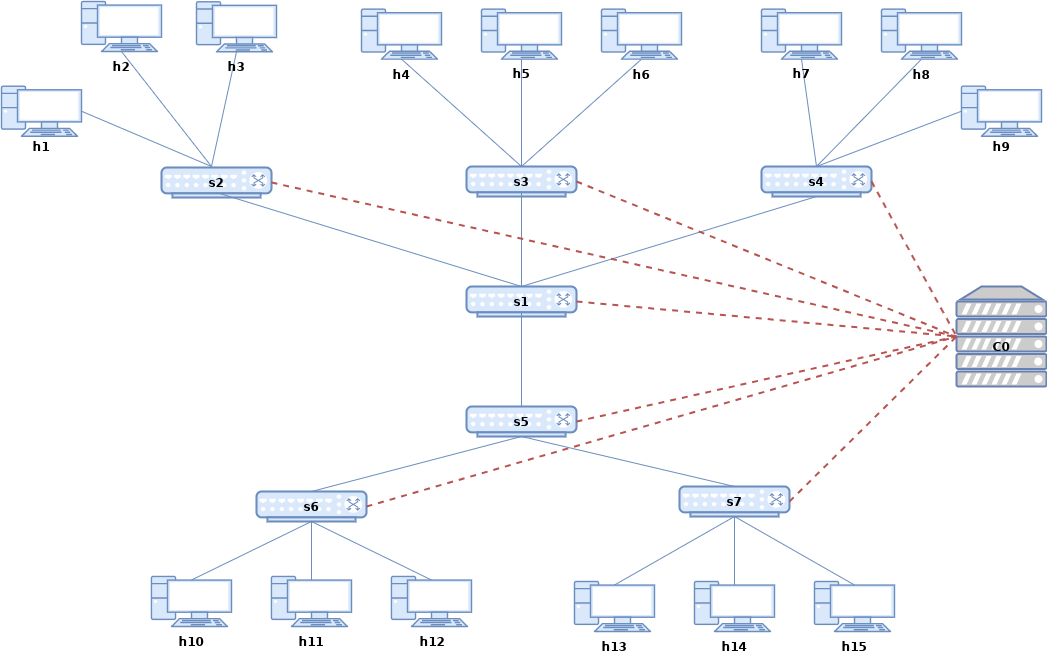
\includegraphics[width=5.5925in,height=3.5091in]{gambar/topologi.png}
\end{center}

Pada topologi diatas adalah topologi yang kami gunakan untuk mengerjakan tugas uas arsitektur jaringan terkini,
dengan menerapkan topologi tree yang menggunakan 15 buah client dan 7 buah switch sebagai penghubung antar clientnya,
untuk mencoba apakah jaringan sudah saling terhubung dan tidak ada kendala pada progress pertama kami menerapkan test
ping pada semua device yang ada apakah ada kesalahan configurasi atau tidak menggunakan perintah \textit{pingall }pada
console mininet dan menghasilkan hasil seperti gambar dibawah ini.


\begin{center}
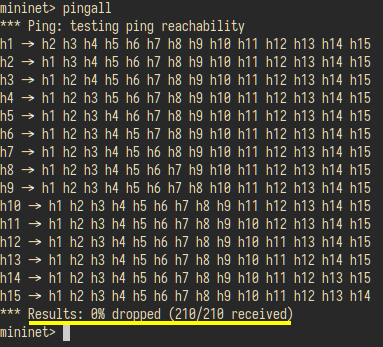
\includegraphics[width=3.989in,height=3.6138in]{gambar/pingall.png}
\end{center}

Dari hasil screenshot diatas dapat diketahui bahwa semua client bisa terkoneksi satu samalain akan tetapi dalam
praktikum aslinya ping hanya bisa dilakukan pada device yang memiliki ip address saja maka dari itu pada pengujian yang
kedua kami melakukan uji coba penambahan ip address pada client yang ada serta menerapkan controler floodlight pada
topologi jaringan yang kami desain. Dengan sebarapan ip address seperti di bawah ini.


\begin{center}
\tablefirsthead{}
\tablehead{}
\tabletail{}
\tablelasttail{}
\begin{supertabular}{|m{1.1087599in}|m{1.7934599in}|}
\hline
\centering{\bfseries Host} &
\centering\arraybslash{\bfseries Ip Address}\\\hline
\centering h1 &
192.168.100.10/27\\\hline
\centering h2 &
192.168.100.11/27\\\hline
\centering h3 &
192.168.100.12/27\\\hline
\centering h4 &
192.168.100.13/27\\\hline
\centering h5 &
192.168.100.14/27\\\hline
\centering h6 &
192.168.100.15/27\\\hline
\centering h7 &
192.168.100.16/27\\\hline
\centering h8 &
192.168.100.17/27\\\hline
\centering h9 &
192.168.100.18/27\\\hline
\centering h10 &
192.168.100.19/27\\\hline
\centering h11 &
192.168.100.20/27\\\hline
\centering h12 &
192.168.100.21/27\\\hline
\centering h13 &
192.168.100.22/27\\\hline
\centering h14 &
192.168.100.23/27\\\hline
\centering h15 &
192.168.100.24/27\\\hline
\end{supertabular}
\end{center}


Setelah configurasi dibuat dengan bahasa pemorgraman python versi 2 maka dilanjutkan untuk uji coba konfigurasi pada
ubuntu 18.04 yang kami gunakan sebagai server mininetnya dengan configurasi terlampir di lembar terakhir. Pada gambar
dibawah ini kami melakukan uji coba test ping dari h1 ke h15 dan dari h1 ke h10.

\begin{center}
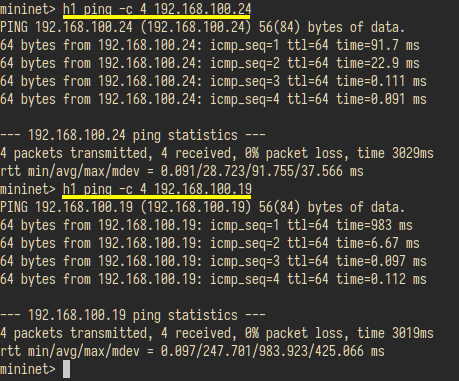
\includegraphics[width=4.7807in,height=3.9681in]{gambar/h1h15h1h10.png}
\end{center}

Pengujian hanya dilakukan pada h1 ke h15 dan h1 ke h10 untuk memberikan gambaran apakah configurasi yang telah kami
buat benar benar berjalan sedangkan hasil pengujian pada semua host yang ada di dalam topologi mininet terlampir di
lembar terakhir setelah lembar configurasi. \\

Setelah tahap pengujian jaringan pada mininet dirasa sudah berhasil selanjutnya kami melakukan pengujian controller
floodlight pada jaringan yang kami buat apakah sudah sesuai dengan keinginan kami atau belum. Tahapan awal yang kami
ambil yakni melakukan instalasi floodlight pada docker container . Docker disini kami fungsikan sebagai host untuk
floodlightnya yang terinstall pada laptop dengan sistem operasi archlinux, sedangkan untuk mininetnya tetap terinstall
di ubuntu 18.04 yang terdapat pada kvm. dibawah ini adalah gambar dari docker container yang sedang menjalankan
floodlight.


\begin{center}
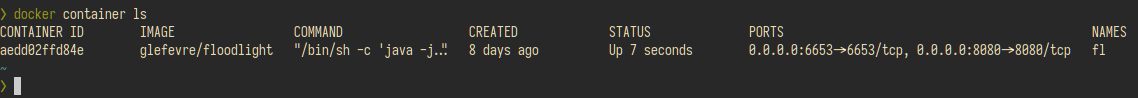
\includegraphics[width=6.9252in,height=0.5957in]{gambar/docker.png}
\end{center}
Setelah tahap pembuatan container pada docker selesai dijalankan, maka web-ui floodlight bisa diakses melalu url
\href{http://localhost:8080/ui/pages/index.html}{ttp://localhost:8080/ui/pages/index.html} untuk melihat tampilan dari
floodlight itu sendiri. Dibawah ini adalah tampilan dari awala floodlight.


\begin{center}
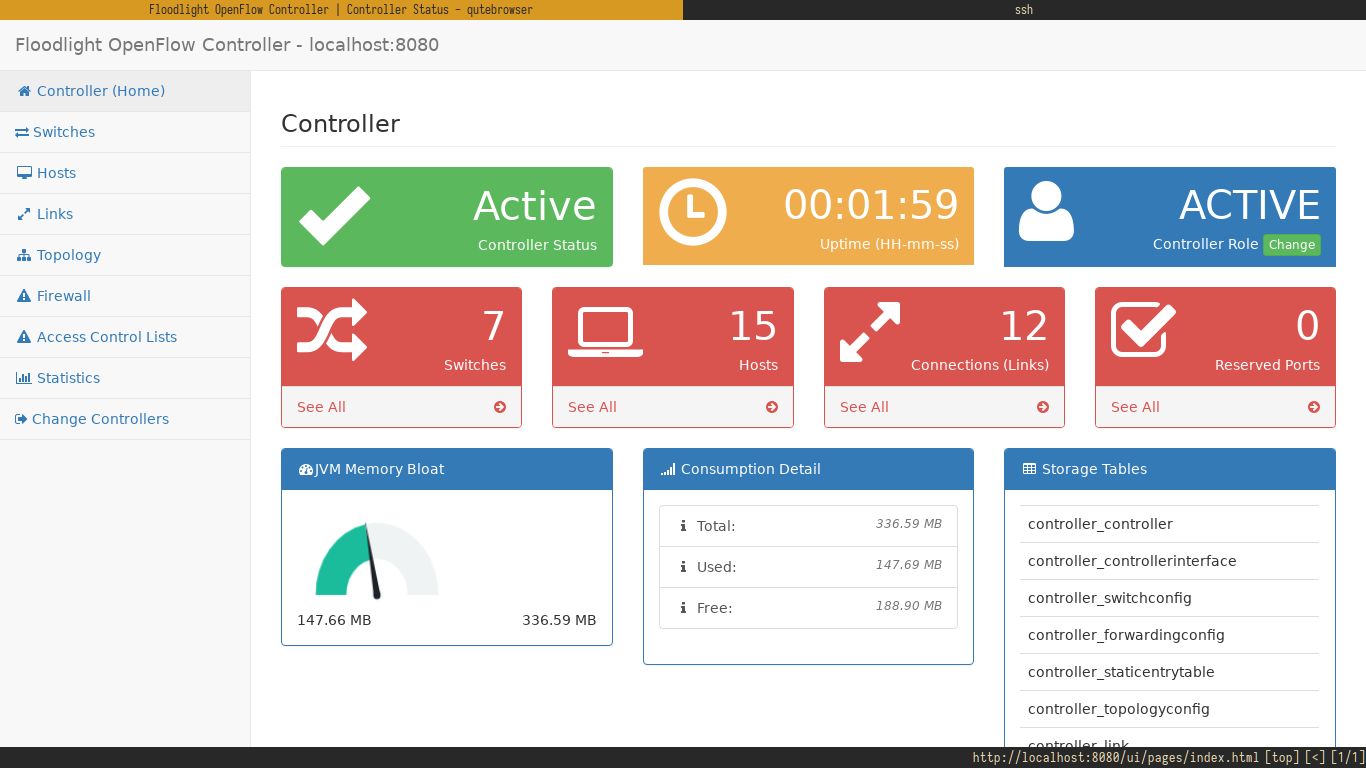
\includegraphics[width=6.9252in,height=3.8827in]{gambar/flhome.png}
\end{center}
Setelah kami rasa floodlight sukses dijalankan maka kami mencoba menjalankan mininet menggunakan floodlight sebagai
controllernya menggunakan perintah.

\bigskip

{\centering
\ sudo mn -{}-custom configurasi.py -{}-topo g1 -{}-controller remote,ip=192.168.122.1,port=6653
\par}

\bigskip

pada perintah diatas dapat diketahui bahwa mininet menggunakan controller floodlight yang memiliki ip address
192.168.122.1 yang mengarah ke interface kvmnya dan berjalan pada port 6653 \ dan menjalankan custom topologi dari
configurasi yang telah kami buat. Dibawah ini adalah console log dari minet ketika dijalankan dengan controller
floodlight.


\begin{center}
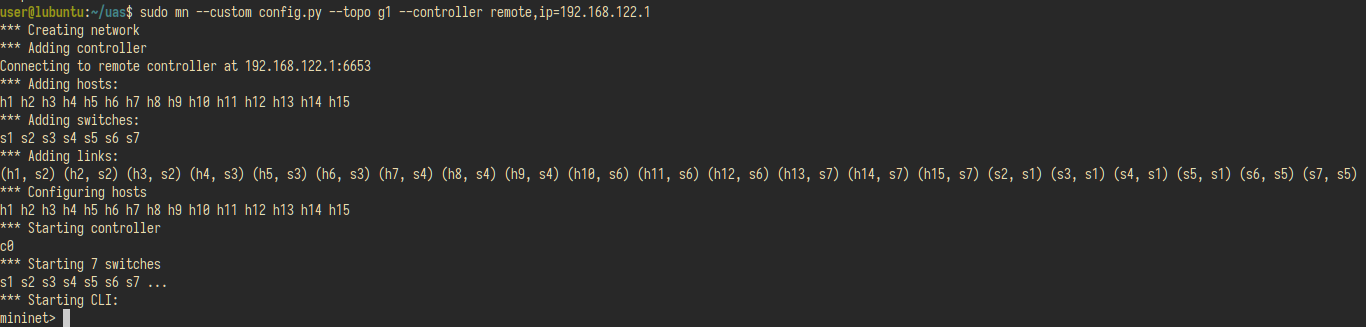
\includegraphics[width=6.9252in,height=1.6575in]{gambar/mininetlog.png}
\end{center}
Pada saat mininet terkoneski dengan controller floodlight kita dapat mengetahui paket apa saja yang dikirimkan dari
mininet ke controller melalui aplikasi wireshark. 

\begin{center}
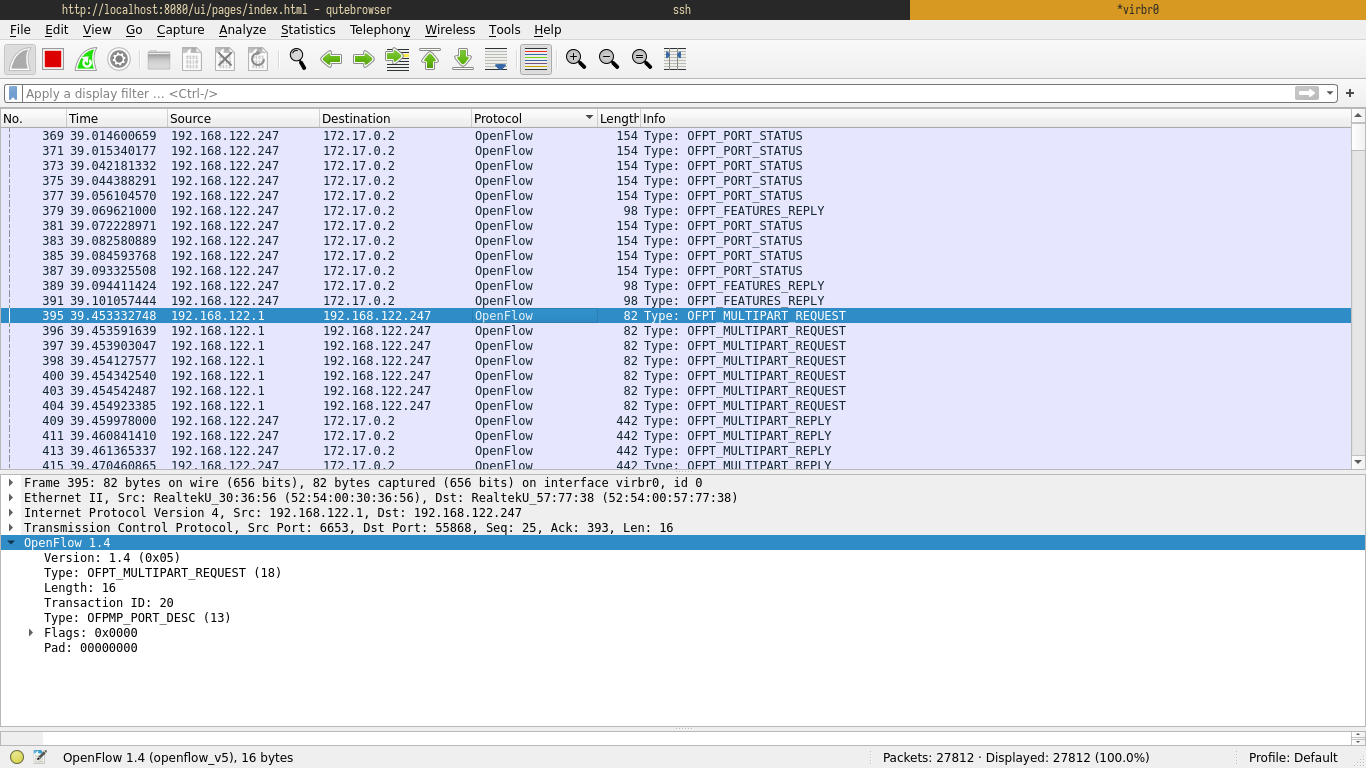
\includegraphics[width=6.9252in,height=3.8929in]{gambar/wireshark.png}
\end{center}

Pada log wireshark di atas ini kita dapat mengetahui bahwa controller floodlight dengan ip address 192.168.122.1
mencoba terkoneksi dengan server mininet yang memiliki ip address 192.168.122.247 dengan cara mengirimkan
\ OFPT\_MULTIPART\_REPLY. Kemudia data yang diterima dari mininet akan ditampilkan ke web-ui floodlight yang bisa
diakses melalui browser pada sistem operasi yang digunakan. Sedangkan untuk melihat topologi pada jaringan mininet bisa
dilihat melalui menu topologi yang ada di web-ui controller floodlight. Gambar dibawah ini adalah gambar ketika
floodlight sukses menampilkan topologi yang ada di mininet.
\begin{center}
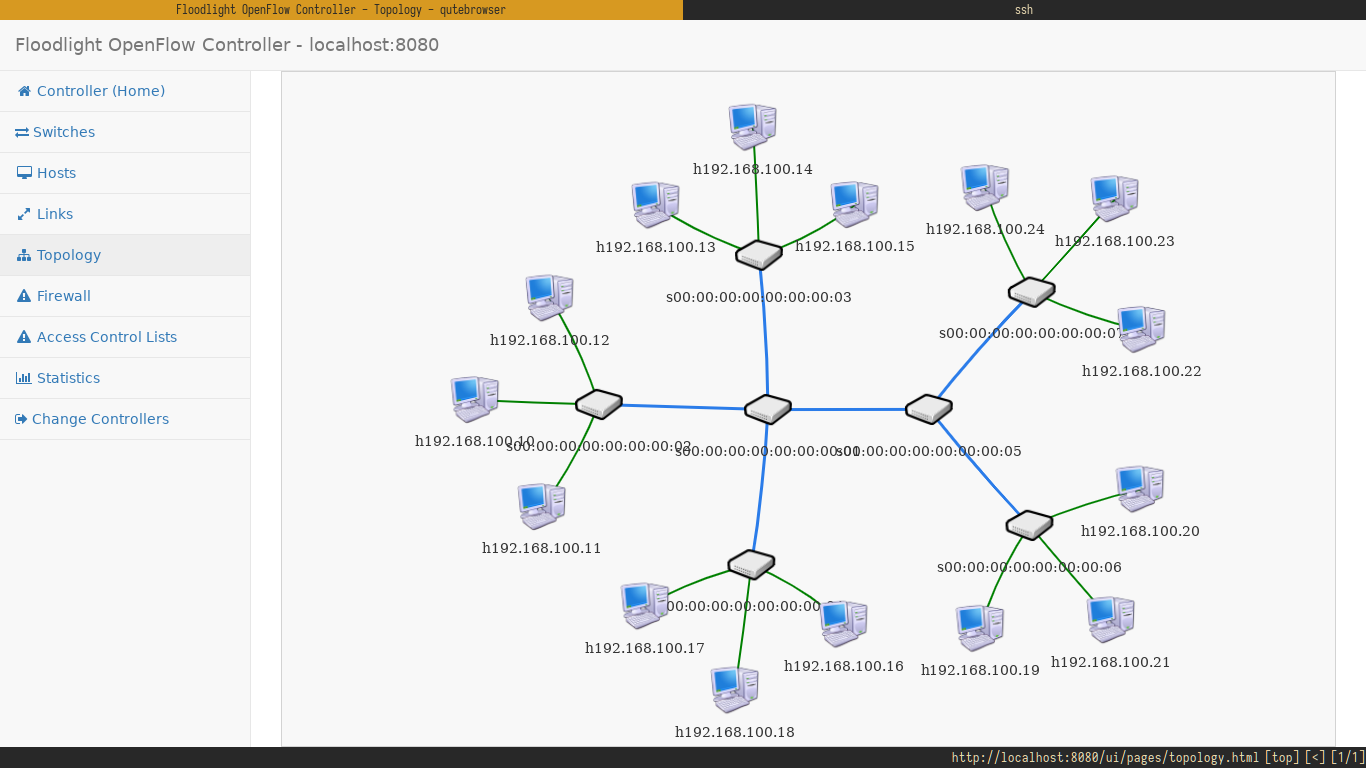
\includegraphics[width=6.9252in,height=3.8929in]{gambar/fltopo.png}
\end{center}
